%\chapter*{} \label{chapitre6-discussion} % "*" pour ne pas afficher le nom de chapitre
\setcounter{section}{0} % 
%\renewcommand*{\theHsection}{chY.\the\value{section}} % version pour la partie méthodes
% See https://tex.stackexchange.com/questions/71162/reset-section-numbering-between-unnumbered-chapters
\renewcommand*{\theHsection}{\theHchapter.\the\value{section}} % différent de l'intro et méthodes, allez savoir pourquoi !

% COVER PAGE
\centerline{\bfseries\textcolor{bleusection}{ \Huge Discussion générale}}  

\bigskip

% Figure cover
\begin{figure}[H] 
	\begin{center}
	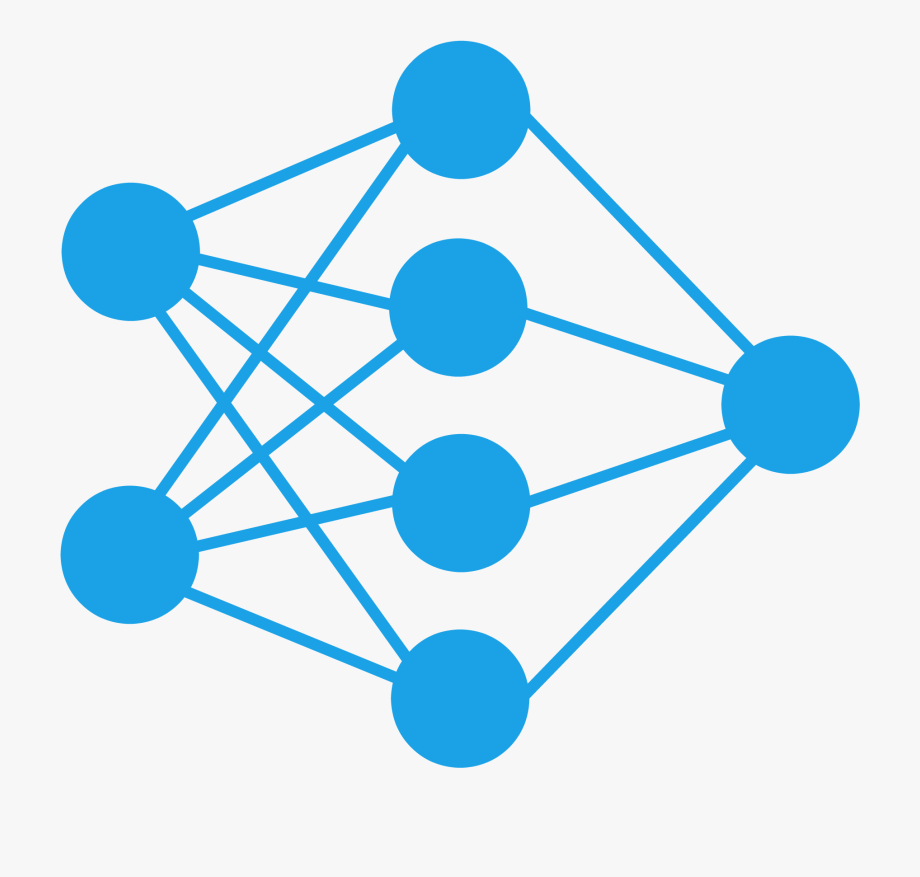
\includegraphics[scale=10]{./7_discussion/cover}
    \end{center}
\end{figure}

% Table des matières intro
{\LARGE
\begin{enumerate}[label=\textcolor{bleusection}{\arabic*}{.}, leftmargin=2cm]
  \item \nameref{discussion.1}
  \item \nameref{discussion.2}
  \item \nameref{discussion.3}
  \item \nameref{discussion.4}
\end{enumerate}
}

\clearpage
\pagestyle{discussion}

\section{Synthèse des résultats}\label{discussion.1}

Cette partie est consacrée à un résumé des messages clés et principaux résultats obtenus au cours de ce travail de recherche doctoral, répondant aux objectifs scientifiques initiaux :

\begin{enumerate}
    \item Développer et entraîner un réseau de neurones convolutifs à reconnaître les espèces du coralligène avec un taux d’erreur semblable ou inférieur à celui d’un expert taxonomiste  (\textbf{\autoref{chapitre1-deep}})~;
    
    \item Définir un protocole d’acquisition plongeur pour réaliser des reconstructions 3D d’habitats marins par photogrammétrie, et quantifier la précision et la résolution de ces reconstructions  (\textbf{\autoref{chapitre2-methode}})~;
    
    \item Développer une méthode de microcartographie automatique des herbiers de posidonie basée sur la photogrammétrie pour permettre un suivi à fine échelle et rapide de la limite inférieure des herbiers  (\textbf{\autoref{chapitre3-herbiers}})~;
    
    \item Caractériser la structure des récifs coralligènes par photogrammétrie et explorer les liens entre structure, composition des assemblages et conditions environnementales (\textbf{\autoref{chapitre4-structure}}).
    
\end{enumerate}

\subsection{Reconnaissance automatique d’espèces des récifs coralligènes par des réseaux de neurones convolutifs}

Dans le \autoref{chapitre1-deep}, nous avons entraîné un ensemble de réseaux de neurones convolutifs à reconnaître les principales espèces des assemblages coralligènes, en bénéficiant de l’importante base de données RECOR (près de 670 000 annotations sur la période 2010 – 2018). Si les performances sont variables d’une classe à l’autre, notamment en fonction de la variabilité intra-classe et de la quantité de vignettes annotées, notre modèle a atteint des performances satisfaisantes avec 72,59 \% de bonnes prédictions sur 61 classes (de niveaux taxonomiques variables). L’analyse multi-échelles des vignettes par notre ensemble de quatre réseaux de neurones a permis d’augmenter la capacité de notre modèle à reconnaître les espèces. Par ailleurs, les confusions sont en partie taxonomiquement cohérentes, car en regroupant les 61 classes en 15 catégories majeures (niveau taxonomique dégradé), les performances atteignent 84,47 \% de bonnes classifications, soit un score supérieur à celui d’un taxonomiste expert sur un problème similaire à 20 classes \citep{beijbom_towards_2015}. Enfin, nous avons développé un outil de classification semi-automatique permettant de valider manuellement les points pour lesquels le niveau de confiance du réseau n’est pas satisfaisant, assurant ainsi une identification de grande précision. En utilisation 100 \% automatique, l’estimation de l’indicateur de Shannon est relativement bonne (coefficient de corrélation de Spearman : 0,74), mais la prédiction du Coralligenous Assemblage Index \citep{deter_preliminary_2012} est moins précise (coefficient de corrélation de Spearman : 0,61), notamment à cause de prédictions erronées sur les bryozoaires et d’une confusion entre les différentes natures de sédiment (vase, sable, détritique).

En considérant la complexité des assemblages coralligènes et les contraintes de notre jeu de données, l’outil développé permet d’atteindre de bonnes performances sur un problème de haut niveau de complexité, et constitue une première brique dans l’utilisation des réseaux de neurones convolutifs pour l’étude des récifs coralligènes. Cependant, l’apprentissage profond est un champ de recherche très dynamique et de nouvelles méthodes sont publiées régulièrement; des développements à venir pourraient bénéficier à notre approche et améliorer les performances ou encore ouvrir vers une segmentation sémantique des quadrats photographiques, permettant d’évaluer précisément le pourcentage de recouvrement de chaque classe. Par ailleurs, les performances par classe étant globalement corrélées au nombre de vignettes disponibles dans le jeu d’entraînement, il est probable que notre modèle affine ses prédictions pour les classes les plus rares à mesure que la base de données s’enrichit lors des prochaines campagnes d’acquisition.

\subsection{Protocole d’acquisition d’images pour la reconstruction 3D d’habitats marins par photogrammétrie}

Dans le \autoref{chapitre2-methode}, nous avons cherché à définir un protocole d’acquisition photogrammétrique « standard » permettant de reconstruire des habitats marins en 3D, en maximisant la qualité des modèles (résolution, précision) tout en minimisant le temps de calcul. En particulier, nous avons évalué l’influence de plusieurs paramètres d’acquisition (type d’appareil photo, altitude de vol, orientation et densité de photos) à travers la réalisation de 192 modèles d’une même zone d’étude. Les résultats ont montré un fort effet de l’appareil photo et de l’altitude de survol sur la qualité des modèles, ces deux facteurs influençant notamment la résolution des pixels de l’image projetés au sol. Quant à la densité de photo, elle permet d’améliorer la précision de l’alignement des images mais au détriment du temps de calcul, qui augmente exponentiellement avec la densité. Concernant l’orientation, nos résultats indiquent qu’il est préférable de réaliser une acquisition avec des photos perpendiculaires à la surface uniquement.

En respectant le protocole d’acquisition déterminé dans cette première expérience, nous avons montré que les modèles 3D obtenus avaient une résolution moyenne de 3,4 mm (distance moyenne entre deux sommets du maillage), soit une densité de points permettant de reproduire la structure centimétrique d’habitats complexes tels que les récifs coralligènes. Par ailleurs, la distance point par point entre la reconstruction d’un rocher artificiel et son modèle hors d’eau très haute définition a montré une grande précision des reconstructions, supérieure à celle mesurée dans d’autres études \citep{figueira_accuracy_2015, bryson_characterization_2017}, avec un écart moyen de l’ordre du millimètre. Enfin, si la précision du positionnement 3D des points reconstruits diminue avec la distance au centre du modèle, l’erreur commise est de l’ordre du centimètre sur une distance de 30 m, soit un niveau de précision largement suffisant pour nos applications cartographiques.

Ce chapitre a permis de définir une méthode simple, rapide, abordable et reproductible pour la reconstruction 3D d’habitats marins par photogrammétrie. Si cette étude est basée sur une zone de taille modeste, et que l’ensemble des résultats n’est pas généralisable à une surface plus grande et plus complexe, les enseignements de cette étude et les ordres de grandeur des résultats permettent de mieux appréhender son utilisation dans le cadre opérationnel des réseaux de surveillance TEMPO et RECOR.

\subsection{Cartographie de la limite inférieure des herbiers de posidonie par photogrammétrie sous-marine}

Dans le \autoref{chapitre3-herbiers}, nous avons développé une méthode de cartographie fine échelle des herbiers de posidonie par photogrammétrie, en bénéficiant de la méthodologie développée au chapitre 2. Si plusieurs études utilisent des orthomosaïques reconstruites à partir d’un modèle photogrammétrique pour cartographier en 2D des habitats benthiques \citep{rende_advances_2015, bonin-font_towards_2016, mizuno_simple_2017}, nous avons imaginé une méthode de cartographie des herbiers qui exploite une limite de la photogrammétrie : l’incapacité à reproduire (précisément) les objets en mouvement. Concrètement, nous avons utilisé le nuage de points épars produit lors de l’alignement des images pour cartographier les zones d’herbiers à partir des espaces ne contenant pas ou trop peu de points 3D. Notre méthode de classification, entraînée sur 21 sites de morphologies et de natures différentes, a obtenu une précision, un taux de rappel et un F1-score moyens de 0,79, 0,91 et 0,84, respectivement. Si nous n’avons pas détecté d’effet du type de substrat (vase ou sable) ni de la densité de feuilles, nous avons montré que la fragmentation de l’herbier avait un effet négatif sur les performances de classification.

L’utilisation de notre méthode sur trois sites de surveillance TEMPO a montré qu’elle permettait de suivre finement l’évolution de la limite inférieure des herbiers de posidonie et d’évaluer leur état de santé par le calcul d’indicateurs surfaciques. Selon la précision cartographique souhaitée et le niveau de fragmentation de l’herbier considéré, il est toujours envisageable de se servir des modèles 3D pour produire les orthomosaïques des sites de surveillance et de numériser manuellement la limite de l’herbier pour plus de précision. Cette méthode est une vraie alternative à la télémétrie acoustique pour la cartographie fine-échelle des herbiers, qui pourrait également être appliquée à d’autres types de végétation ou d’algues en exploitant le même principe mais en réajustant les paramètres.

\subsection{Caractérisation de la structure des récifs coralligènes et liens entre structure et composition des assemblages}

Dans le \autoref{chapitre4-structure}, nous avons utilisé la photogrammétrie pour caractériser la structure tridimensionnelle des récifs coralligènes et explorer les liens entre structure et composition des assemblages. Sur la base des 39 reconstructions 3D, nous avons calculé plusieurs indicateurs caractérisant la forme et la complexité des récifs : dimension fractale et rugosité à plusieurs échelles. À partir de ces indicateurs, nous avons déterminé quatre morphologies de récifs : les récifs peu complexes, les récifs moyennement complexes avec des structures de — petite ou de grande — taille, et enfin les récifs les plus complexes. 

En ce qui concerne les assemblages écologiques, nous n’avons pas détecté de différences significatives de composition entre les différents morphotypes. Notamment, nous n’avons pas observé de corrélation entre la complexité structurale des récifs et la diversité des assemblages ou leur état écologique, comme certaines études semblent le suggérer en milieu corallien \citep{darling_relationships_2017, burns_3d_2019, price_using_2019, carlot_community_2020}. Nous avons avancé trois hypothèses pour expliquer ces résultats : premièrement, si pour chaque récif les quadrats photographiques sont réalisés sur la zone numérisée par photogrammétrie, nous n’avons pas pu localiser précisément les quadrats et il se pourrait que le ratio des surfaces échantillonnées par quadrats et par photogrammétrie ne permette pas de tisser de réels liens entre la structure et la composition des assemblages. En effet, les acquisitions photogrammétriques ont été ajoutées aux méthodes déjà utilisées dans le cadre du réseau RECOR, et l’échantillonnage est probablement une cause non négligeable de variance dans la donnée. Pour explorer les liens entre structure et composition des assemblages, il serait préférable de les étudier à plus fine échelle, en réalisant des inventaires naturalistes plus exhaustifs et localisés sur la surface 3D comme cela l’a été fait dans d’autres études \citep{price_using_2019}, afin de corréler à la structure locale du récif. Deuxièmement, les récifs coralligènes sont des récifs profonds, généralement très peu exposés aux contraintes mécaniques des tempêtes en surface, contrairement aux récifs coralliens dont la dynamique structurale est directement affectée par les tempêtes tropicales et les épisodes de blanchiment. Ainsi, la structure des récifs coralliens serait globalement corrélée aux assemblages qui les composent à un instant t, tandis que la structure des récifs coralligènes pourrait être davantage le reflet de leur histoire que de leur état actuel. Certains des récifs du réseau RECOR étayent cette hypothèse : ils ont une structure complexe, fruit de nombreuses décennies de concrétions \citep{sartoretto_age_1996}, mais sont aujourd’hui en mauvais état de santé avec une biodiversité fixée érodée par la sédimentation et une mauvaise qualité de l’eau \citep{airoldi_effects_2003, holon_predictive_2018}. Enfin, les récifs coralligènes sont d’une grande complexité écologique et la composition des assemblages peut être très hétérogène, y compris à une échelle très locale \citep{kipson_rapid_2011}. Il est probable que l’étude et la compréhension des interactions entre structure et composition des assemblages nécessitent un nombre largement supérieur de sites échantillonnés.

\section{Vers une surveillance efficace des habitats marins en Méditerranée française}\label{discussion.2}

Dans le contexte actuel de changement global et des effets des pressions anthropiques sur les mers et les océans, un des principaux enjeux de la surveillance de l’état écologique des habitats marins est l’\textbf{accessibilité à une donnée fine et précise} sur la répartition et la composition des assemblages à l’échelle régionale. Il existe donc des \textbf{besoins méthodologiques} permettant la \textbf{collecte} et le \textbf{traitement} de grands volumes de données, dont les résultats doivent être \textbf{interprétés} et \textbf{synthétisés} pour assister les gestionnaires dans \textbf{l’élaboration de mesures de conservation efficaces}. L’objectif principal de cette thèse CIFRE était de répondre à ces besoins méthodologiques par le \textbf{développement de méthodes opérationnelles} basées sur la \textbf{photogrammétrie} et l’analyse d’images, pour caractériser et suivre l’\textbf{évolution de la biodiversité} marine méditerranéenne. En bénéficiant notamment des campagnes de terrain opérées par Andromède Océanologie dans le cadre des réseaux de surveillance RECOR et TEMPO, nous avons pu acquérir les données nécessaires au développement de nouvelles méthodes qui seront à terme intégrées à ces réseaux et aux autres études de la société.

\subsection{Caractérisation et suivi de l’état écologique des récifs coralligènes}

D’une richesse spécifique semblable aux récifs coralliens, les récifs coralligènes font partie des deux habitats les plus riches et sensibles de Méditerranée \citep{boudouresque_marine_2004}. Pourtant, ils sont directement et indirectement soumis à un certain nombre de pressions anthropiques côtières, c’est pourquoi le réseau de surveillance RECOR a été initié en 2010 afin de suivre la composition des assemblages coralligènes à l’échelle de la façade méditerranéenne française. Comme mentionné en introduction et dans le \autoref{chapitre1-deep}, l’étude et le suivi des récifs coralligènes à l’échelle régionale est extrêmement coûteuse en temps, car elle nécessite l’analyse experte de nombreux quadrats photographiques pour identifier les espèces observées \citep{kipson_rapid_2011, deter_rapid_2012, sartoretto_integrated_2017}. L’entraînement d’un ensemble de réseaux de neurones avec des performances proches de celles d’un expert taxonomiste rend envisageable son utilisation de manière opérationnelle pour réaliser les annotations à venir, et pourrait également permettre d’intensifier l’effort d’échantillonnage aussi bien en termes de nombre de points identifiés par récif qu’en nombre de récifs suivis \citep{beijbom_towards_2015}. Compte tenu de la grande diversité et variabilité dans la composition de ces assemblages \citep{kipson_rapid_2011}, il est en effet nécessaire de suivre un grand nombre de sites afin de comprendre ce qui structure ces assemblages et conditionne leur état écologique pour mieux aviser les gestionnaires. Par ailleurs, si le réseau n’est pas capable de prédire une classe qu’il n’a pas apprise, l’outil de classification sélective permet de classer les images dont il est le plus sûr, avec un taux d’erreur connu, en laissant les images plus incertaines ou dont il ne connaît pas la classe à annoter par un taxonomiste expert. Nous avons ainsi commencé à développer une interface graphique permettant au taxonomiste de charger les images, choisir le taux d’erreur acceptable et lancer la classification (\autoref{figure_discussion1}). A l’image de CoralNet (\href{https://coralnet.ucsd.edu/}{https://coralnet.ucsd.edu/}) \citep{beijbom_towards_2015}, cette interface pourrait à terme être mise en ligne et bénéficier à tout utilisateur, scientifique ou gestionnaire, afin d’annoter automatiquement les images sous-marines de récifs coralligènes et de contribuer à la base de données RECOR.

%%%%%%%%%%%%%%%%%%%%%%%%%%%%%%%%%%%%%%%%%%%%%%%
%%% Figure discussion 1: interface coradeep %%%
%%%%%%%%%%%%%%%%%%%%%%%%%%%%%%%%%%%%%%%%%%%%%%%
\begin{figure}[H]
	\begin{center}
	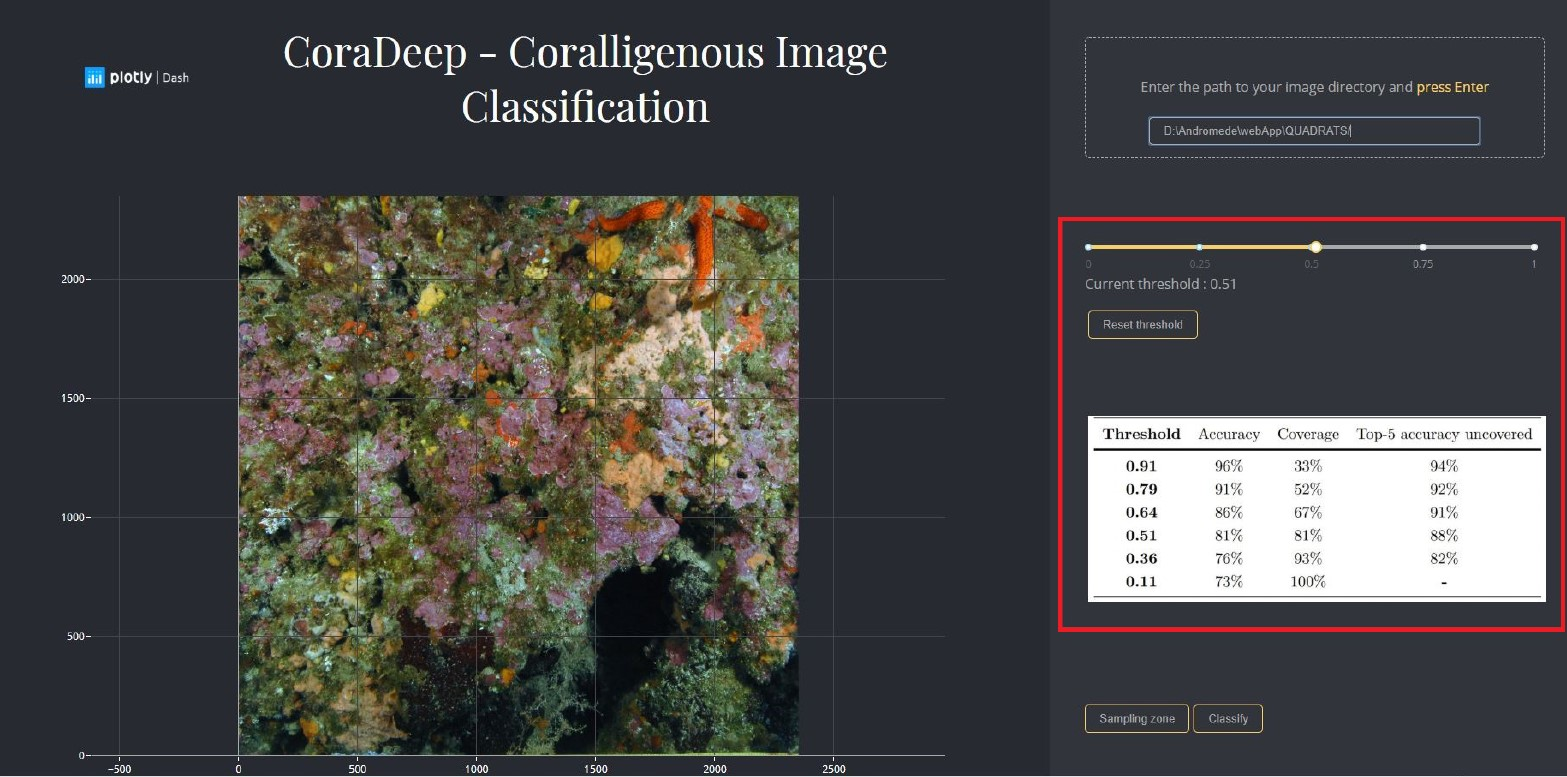
\includegraphics[width=\linewidth,keepaspectratio]{./7_discussion/coradeep}
		\caption{Interface graphique de l’outil d’annotation semi-automatique des images de récifs coralligènes.}
	\label{figure_discussion1}
\end{center}
\end{figure}

À défaut de liens probants entre la structure des récifs et leur état écologique, la photogrammétrie permet de reproduire l’état d’un récif à un instant donné, et d’un suivi à l’autre, d’aligner les modèles 3D et de visualiser, localiser et quantifier les différences. Si certaines différences morphologiques, notamment dues à la croissance, nécessitent une précision de reconstruction certainement supérieure à celle de notre méthode (croissance très faible des récifs coralligènes \citep{sartoretto_age_1996}, artefacts dus à la présence d’algues filamenteuses, ombres portées…), il est en revanche possible de produire des vues identiques sur le récif aux différents pas de temps et de mesurer par exemple l’extension ou la régression d’une zone de nécrose (\autoref{figure_discussion2}).

%%%%%%%%%%%%%%%%%%%%%%%%%%%%%%%%%%%%%%%%%%%%%
%%% Figure discussion 2: suivis temporels %%%
%%%%%%%%%%%%%%%%%%%%%%%%%%%%%%%%%%%%%%%%%%%%%
\begin{figure}[H]
	\begin{center}
	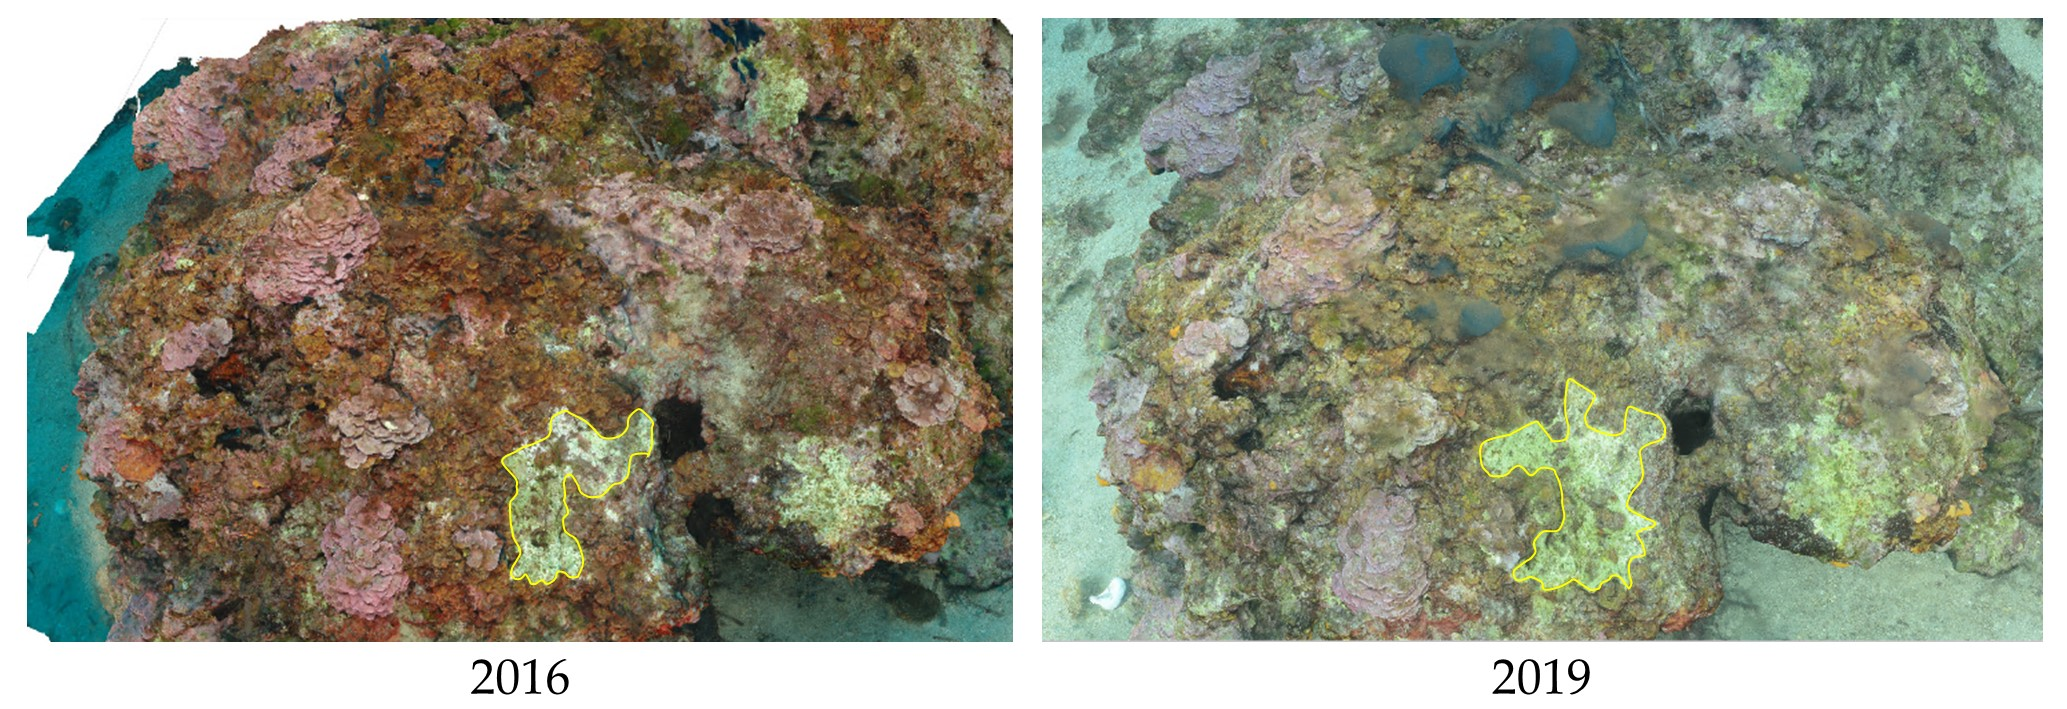
\includegraphics[width=\linewidth,keepaspectratio]{./7_discussion/RECOR_temporel}
		\caption{Extension d’une nécrose d’algues rouges encroûtantes sur le site « Rade de Bormes » à partir des modèles 3D de 2016 et 2019.}
	\label{figure_discussion2}
\end{center}
\end{figure}

De manière générale, il est envisageable de définir un certain nombre de zones d’intérêt sur le récif et de produire pour chaque nouveau modèle les orthomosaïques locales correspondantes pour suivre l’évolution individuelle de nombreux points sur le récif et s’affranchir de l’aspect aléatoire de l’échantillonnage actuel par quadrats photographiques (compensé par le nombre suffisant de points identifiés). C’est ce que nous avons mis en place dans le cadre du suivi de la recolonisation d’un récif à Saint-Jean-Cap-Ferrat, nettoyé en 2018 (retrait de sédiment), pour lequel nous suivons régulièrement 14 quadrats permanents de surface ~1 m² répartis sur la partie restaurée et la partie intacte du récif. A chaque suivi, nous réalisons un modèle photogrammétrique à partir duquel nous reproduisons les orthomosaïques locales au droit de chaque quadrat. Cette méthode permet de superposer précisément les orthomosaïques locales d’un suivi à l’autre et de suivre finement la recolonisation du récif (\autoref{figure_discussion3}). Ce type d’analyses pourrait être intégré aux suivis RECOR afin de quantifier précisément l’évolution d’observations singulières telles que les nécroses.

%%%%%%%%%%%%%%%%%%%%%%%%%%%%%%%%%%%%%%%%%%%%%%%%
%%% Figure discussion 3: quadrats permanents %%%
%%%%%%%%%%%%%%%%%%%%%%%%%%%%%%%%%%%%%%%%%%%%%%%%
\begin{figure}[H]
	\begin{center}
	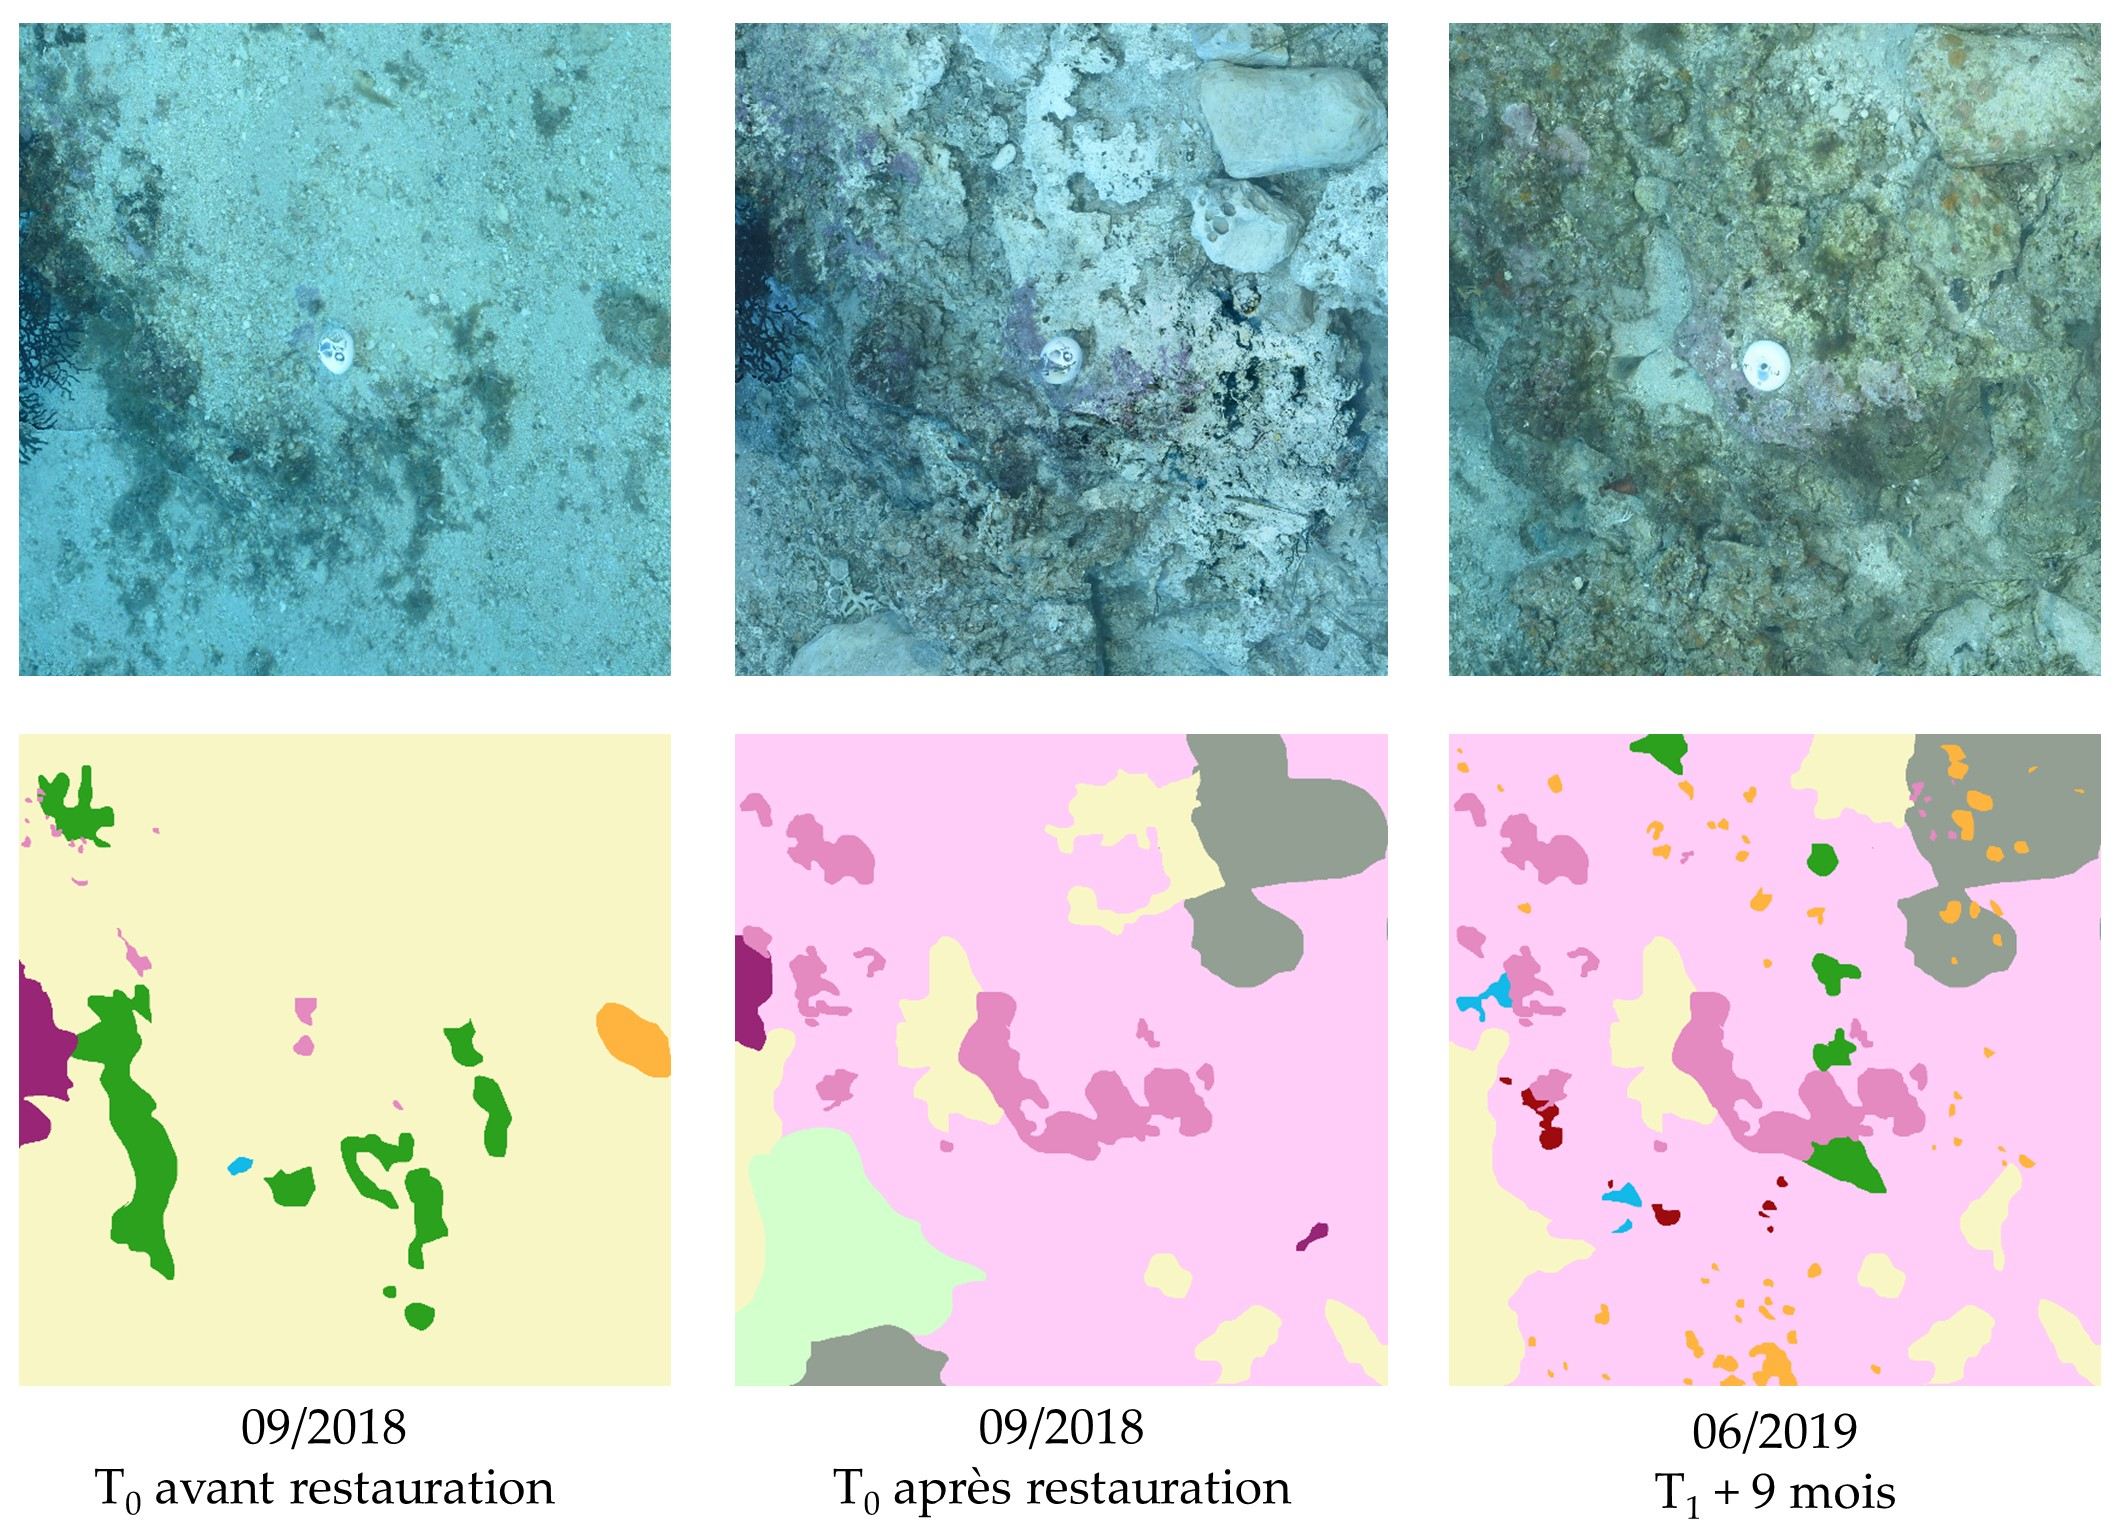
\includegraphics[width=\linewidth,keepaspectratio]{./7_discussion/quadrats_permanents}
		\caption[Suivi photogrammétrique de la recolonisation d’un récif coralligène à Saint-Jean-Cap-Ferrat après restauration]{Suivi photogrammétrique de la recolonisation d’un récif coralligène à Saint-Jean-Cap-Ferrat après restauration. Gris = substrat rocheux ; jaune pâle = substrat meuble ; vert foncé = algues ; vert clair = débris biologiques ; rose pâle = coralligène nécrosé ; rose foncé = corallinacées ; orange = bryozoaires ; bleu = vivant non identifié ; violet pourpre = gorgones.}
	\label{figure_discussion3}
\end{center}
\end{figure}

Concernant la structure des récifs coralligènes, le \autoref{chapitre4-structure} constitue un travail exploratoire, qui jette les bases de la réflexion sur les liens entre structure et état écologique. A ce stade, la prise en compte de la structure dans le réseau RECOR nécessite de poursuivre les travaux de recherche, notamment en explorant les relations à plus fine échelle en localisant les annotations sur le modèle 3D \citep{price_using_2019}. Quel que soit l’indicateur structural choisi, s’il advenait que la structure était davantage un héritage évolutif que le reflet d’un état écologique présent, cela permettrait de définir un nouvel indicateur d’état de santé en quantifiant l’écart entre diversité écologique actuelle et structure héritée. Quoiqu’il en soit, les \textbf{acquisitions photogrammétriques} sont désormais \textbf{intégrées au réseau RECOR}, et les données 3D collectées lors des prochaines campagnes permettront d’alimenter la recherche sur cet habitat aussi fragile que complexe.

\subsection{Caractérisation et suivi de l’état écologique des herbiers de posidonie}

Habitat reconnu « d’intérêt spécifique » en termes de biodiversité, les herbiers de posidonie remplissent de nombreux services écosystémiques dont nous dépendons \citep{millenium_ecosystem_assessment_ecosystem_2005, ipbes_global_2019}. Pourtant, cet habitat fragile est soumis à de nombreuses pressions anthropiques \citep{holon_impact_2015}. C’est pourquoi le réseau TEMPO a démarré en 2011, afin de suivre l’évolution de la qualité écologique des herbiers le long de la façade méditerranéenne française et de conseiller les gestionnaires pour préserver cet habitat sensible. Cependant, la détection de ces évolutions nécessite de cartographier à fine échelle la limite inférieure des herbiers, aujourd’hui réalisée par télémétrie acoustique. Si cette technique est reconnue pour sa précision \citep{descamp_underwater_2005, descamp_fast_2011}, elle est couteuse en temps passé sous l’eau et la résolution des polygones dessinés par l’opérateur est dépendante de sa bonne volonté. La méthode que nous avons développée et discutée au \autoref{chapitre3-herbiers}, basée sur la photogrammétrie sous-marine, a des performances suffisantes pour cartographier avec précision les sites présentant un herbier peu fragmenté. En revanche, la précision dégradée dans le cas d’herbiers trop fragmentés pourrait ne pas satisfaire l’exigence d’un réseau de surveillance tel que TEMPO. Mais la photogrammétrie permet de reconstituer une orthomosaïque de la limite qui peut être ensuite utilisée pour numériser manuellement l’herbier à l’aide d’un logiciel de cartographie. Que la cartographie soit réalisée par classification automatique ou par numérisation manuelle, la photogrammétrie permet d’acquérir rapidement une donnée d’une grande précision et dont le temps d’acquisition est indépendant de la fragmentation de l’herbier, contrairement à la télémétrie. Les \textbf{acquisitions photogrammétriques} sont aujourd’hui \textbf{intégrées au réseau TEMPO} en limite inférieure, et les données acquises lors des prochaines campagnes pourront être utilisées pour de futurs développements cartographiques permettant de mieux suivre cet habitat sensible.

\medskip 

\setlength{\fboxsep}{5pt}
\setlength{\fboxrule}{0.6pt}
\noindent\framebox{%
  \begin{minipage}{\linewidth}
    Compte tenu de la \textbf{difficulté et du coût d’accès} au monde sous-marin, la surveillance des habitats marins nécessite de \textbf{développer des méthodes} d’observation \textbf{innovantes} et \textbf{abordables} permettant d’évaluer et de suivre précisément leur \textbf{état écologique}. Ce travail de thèse a permis de développer des \textbf{méthodes opérationnelles} de suivis écologiques des herbiers de posidonie et des récifs coralligènes qui viennent aujourd’hui compléter les \textbf{protocoles d’acquisition} et de \textbf{traitement} de données des réseaux de surveillance TEMPO et RECOR.
  \end{minipage}
}

\section{Perspectives de recherches pour l’amélioration de la surveillance marine}\label{discussion.3}

Si ce travail de recherche a permis de répondre à certains besoins méthodologiques à une surveillance efficace des herbiers de posidonie et des récifs coralligènes, les résultats obtenus ouvrent des perspectives sur de nouvelles questions de recherches et de développements innovants permettant d’y répondre. Les résultats mitigés sur les interactions entre structure des récifs coralligènes et les assemblages correspondants soulèvent le problème de la méthode d’échantillonnage des assemblages relativement aux zones numérisées en 3D par photogrammétrie. Explorer plus en profondeur ces relations demande de pouvoir échantillonner les espèces directement sur le modèle 3D pour associer assemblages locaux aux indicateurs structurels locaux. Par ailleurs, il serait intéressant d’étudier les liens entre la structure des récifs, les espèces fixées et les espèces mobiles, afin de vérifier si la structure influence aussi la diversité et l’abondance d’espèces mobiles comme c’est le cas en milieu corallien. D’autre part, certaines dynamiques écologiques peuvent nécessiter des microcartographies ou des reconstructions 3D sur des zones plus étendues que celles réalisées dans le cadre de ce travail. Or plus la zone à couvrir est grande, plus il est difficile pour le plongeur de conserver une trajectoire optimale permettant d’assurer le bon recouvrement de l’ensemble de la zone. Un outil plongeur en fin de développement devrait permettre de pallier cette limitation. Enfin, si nous avons exclusivement travaillé sur deux habitats méditerranéens, certains résultats et méthodes pourraient être transférés et appliqués à d’autres habitats, notamment les récifs coralliens.

\subsection{Affiner l’étude des liens entre la structure des récifs coralligènes et la composition locale des assemblages}

Comme nous l’avons déjà mentionné plus haut, les résultats nuancés du chapitre 4 souffrent d’une variabilité partiellement induite par le fait que nous n’avons pas pu repositionner les observations sur les modèles 3D, comme ce qui a été fait dans d’autres études en milieu corallien \citep{burns_3d_2019, price_using_2019, carlot_community_2020}. S’il nous est désormais possible de reconnaître automatiquement les principales espèces du coralligène sur des quadrats photographiques et de reconstruire des récifs en 3D par photogrammétrie, il manque aujourd’hui un outil permettant de cartographier automatiquement les espèces sur les modèles 3D pour étudier localement le lien entre assemblages et structure. Par ailleurs, si nous étions en mesure de reconnaître et cartographier en 3D les espèces des assemblages coralligènes, il suffirait d’une acquisition photogrammétrique de qualité pour calculer automatiquement un ensemble d’indicateurs décrivant l’état du récif : biodiversité, état écologique, pourcentage d’envasement, nombre de cavités, surface 3D… 

La photogrammétrie permet de faire le lien entre un point 3D et les coordonnées 2D de l’ensemble des images sur lesquelles il apparaît, et inversement, à partir de coordonnées 2D sur une image, d’obtenir le point 3D sur la surface visible. Il serait donc envisageable de sélectionner aléatoirement un grand nombre de points sur la surface d’un récif, et pour chaque point, extraire l’ensemble des vignettes correspondantes centrées sur ce point et les identifier à l’aide de l’ensemble de réseaux de neurones. Malheureusement, les quadrats photographiques à partir desquels a été entraîné notre modèle sont réalisés à une distance réduite du récif (< 0,5 m), alors que les acquisitions photogrammétriques sont réalisées à environ 1,5 m de distance du récif pour avoir une fauchée et un recouvrement suffisants. Les images sont donc de natures (couleurs, résolution) très différentes, et les performances du modèle chutent considérablement sur un jeu de données test (31,85 \% de bonnes classifications sur environ 5000 points 3D annotés, au lieu des 72,59 \% sur les quadrats photographiques). Il est cependant envisageable d’ajuster notre modèle existant pour le rendre capable d’analyser les images de la photogrammétrie, par un processus dit « d’adaptation de domaine » \citep{goodfellow_deep_2016}. Le principal problème est que nous disposons d’assez peu de points 3D annotés pour réaliser cette adaptation, mais une technique ayant fait ses preuves sur plusieurs jeux de données utilise des Generative Adversarial Networks pour augmenter les données et conserver de bonnes performances après adaptation malgré un nouveau jeu de données de taille modeste \citep{antoniou_data_2018}. Dans la mesure où cette adaptation obtiendrait des performances satisfaisantes, il serait par ailleurs envisageable de bénéficier des différentes prises de vue de chaque point 3D pour rendre la prédiction plus robuste en moyennant par exemple les scores pour chaque vignette (\autoref{figure_discussion4}). De premiers essais sur le jeu de 5000 points 3D et l’ensemble de réseaux actuel ont montré une amélioration des prédictions de l’ordre de 2 \%, mais ce gain pourrait être supérieur sur un réseau d’abord adapté aux images de la photogrammétrie. Par ailleurs, il est possible d’accéder à l’information de profondeur pour chaque pixel de l’image (distance à la surface 3D) afin de ne conserver que les vignettes extraites de photos prises à une distance acceptable du récif.

%%%%%%%%%%%%%%%%%%%%%%%%%%%%%%%%%%%%%%%%%%%%%
%%% Figure discussion 4: couplage deep PG %%%
%%%%%%%%%%%%%%%%%%%%%%%%%%%%%%%%%%%%%%%%%%%%%
\begin{sidewaysfigure}
\begin{figure}[H]
	\begin{center}
	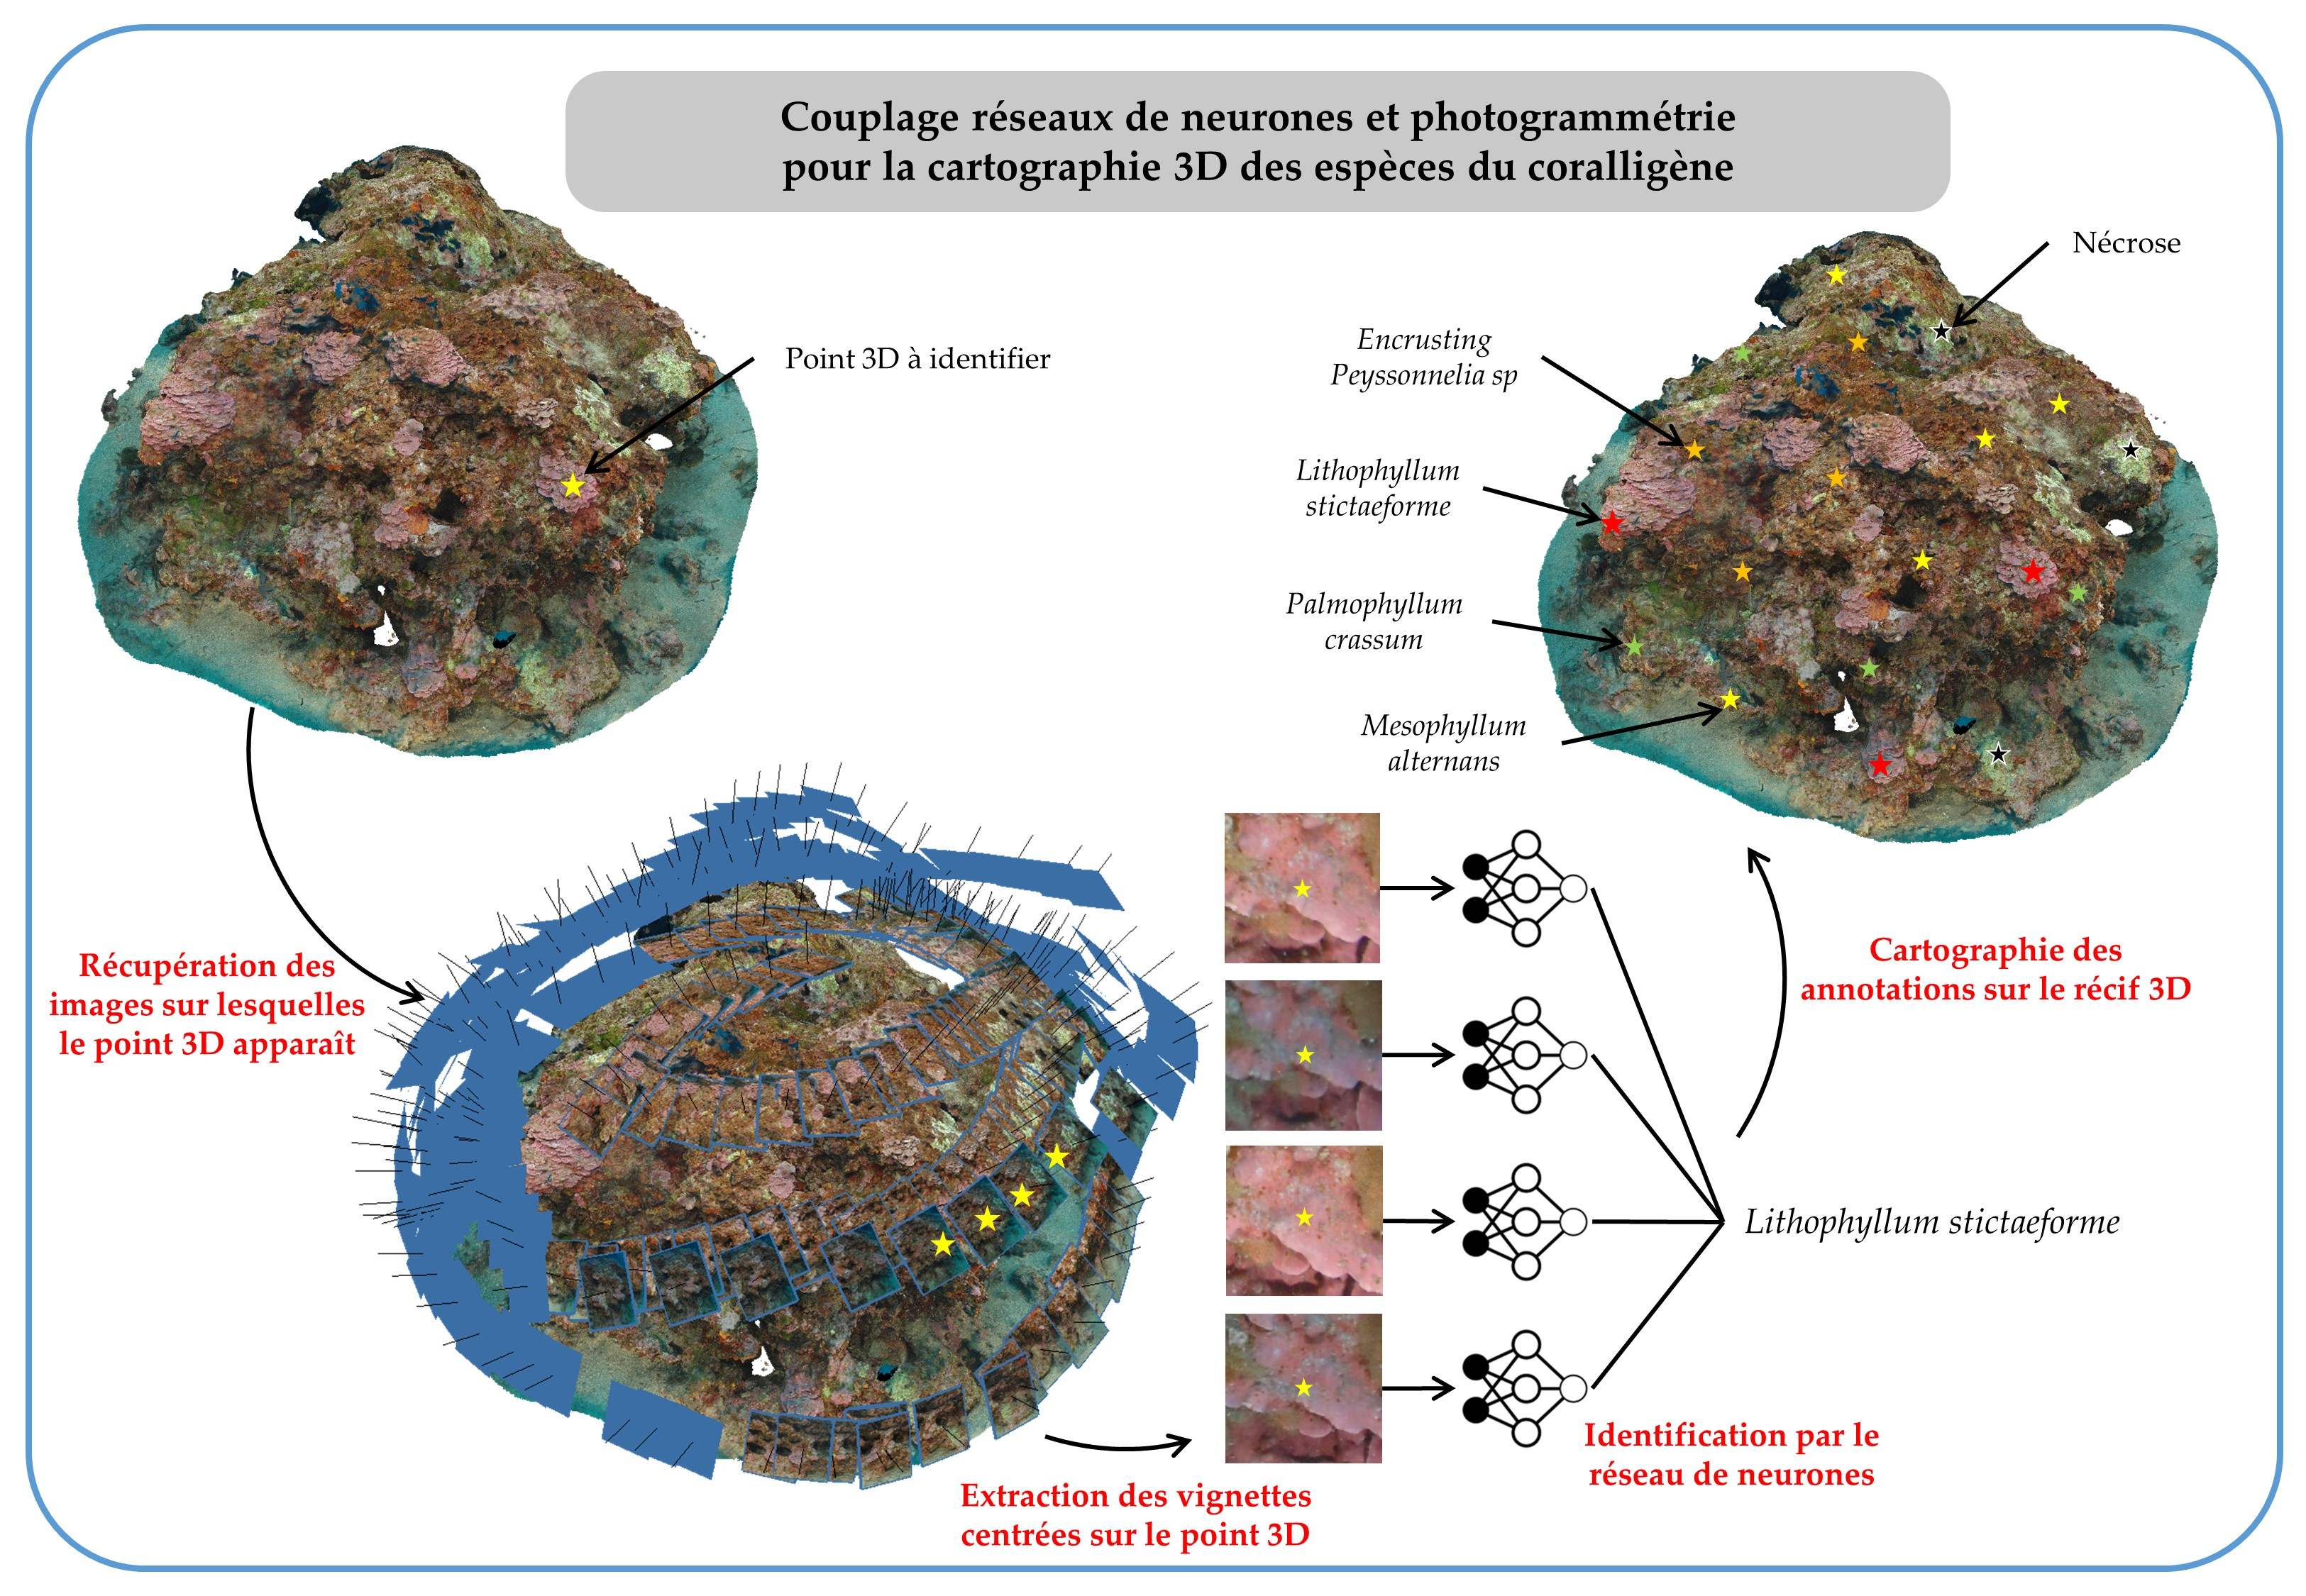
\includegraphics[width=\linewidth,keepaspectratio]{./7_discussion/couplage_deep_PG}
		\caption{Cartographie 3D automatique des espèces du coralligène par couplage photogrammétrie et réseaux de neurones convolutifs.}
	\label{figure_discussion4}
\end{center}
\end{figure}
\end{sidewaysfigure}

D’autre part, une piste alternative d’étude des liens entre structure et diversité des assemblages visait à adapter une méthode d’évaluation de la biodiversité des forêts tropicales par l’analyse d’images hyperspectrales \citep{feret_mapping_2014} en segmentant le nuage de points dense en « espèces structurales » à partir des propriétés géométriques locales (\autoref{figure_discussion5}), afin de calculer des indicateurs de diversité tels que l’indice de Shannon. Si cette méthode n’a pas permis d’expliquer davantage la diversité des assemblages, elle constitue une approche intéressante de la diversité structurale qui mérite davantage d’investigation, notamment en couplant le résultat de ces segmentations avec le positionnement d’espèces par la méthode ci-dessus.

%%%%%%%%%%%%%%%%%%%%%%%%%%%%%%%%%%%%%%%%%%%%%
%%% Figure discussion 5: méthode JB Féret %%%
%%%%%%%%%%%%%%%%%%%%%%%%%%%%%%%%%%%%%%%%%%%%%
\begin{figure}[H]
	\begin{center}
	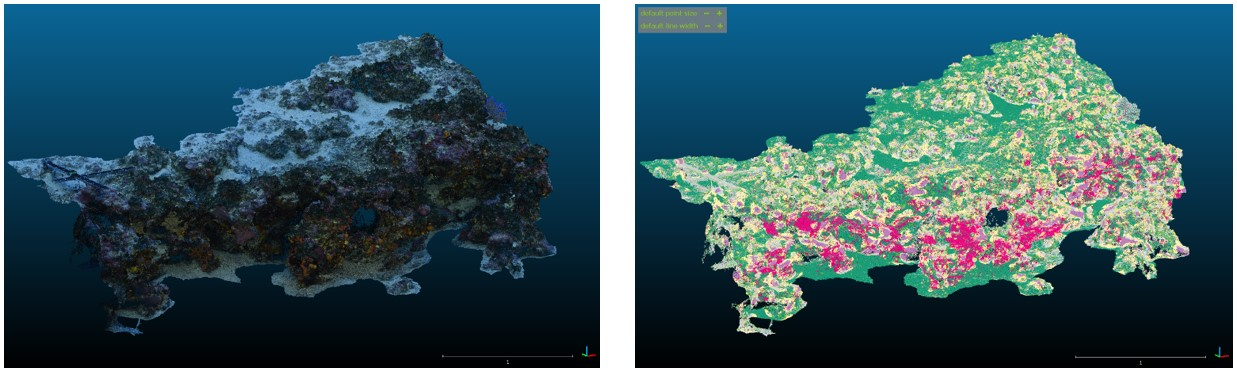
\includegraphics[width=\linewidth,keepaspectratio]{./7_discussion/segmentation_3D}
		\caption[Segmentation du nuage de points 3D d’un récif coralligène sur la base de leur morphologie locale]{Segmentation du nuage de points 3D d’un récif coralligène sur la base de leur morphologie locale. À gauche : récif texturé en couleurs naturelles ; à droite : récif coloré en fonction de zones morphologiquement similaires.}
	\label{figure_discussion5}
\end{center}
\end{figure}

\subsection{Étude des interactions entre structure, biodiversité fixée et biodiversité mobile des récifs coralligènes}

Au cours de ce travail de thèse, nous n’avons malheureusement pas pu prendre en compte la composante « espèces mobiles » dans nos analyses, notamment les interactions entre diversité et abondance de poissons avec la structure des récifs coralligènes, comme d’autres études l’ont montré en milieu corallien \citep{willis_habitat_2005, graham_importance_2013, darling_relationships_2017, price_using_2019}. Comme mentionné en introduction, le réseau CALME (en partenariat avec l’équipe de Chorus : \href{https://chorusacoustics.com/}{https://chorusacoustics.com/}) bancarise des mesures bioacoustiques sur certains sites TEMPO et RECOR afin de quantifier l’activité des espèces mobiles. Si ces mesures sont réalisées avec un seul capteur et sont donc omnidirectionnelles, l’équipe Chorus a développé des algorithmes de traitement du signal permettant de localiser la direction et l’intensité d’un son à partir d’un réseau de quatre hydrophones. En se positionnant face à un récif, ou au-dessus d’un récif, il est ainsi possible de produire une cartographie de l’activité acoustique des différents compartiments vivants du récif (notamment les poissons et les invertébrés benthiques). En réalisant ce type de mesures sur un nombre suffisant de récifs, conjointement à une acquisition photogrammétrique, et en bénéficiant d’un réseau de neurones adapté aux images de la photogrammétrie pour cartographier les espèces fixées sur le modèle 3D (voir sous-section précédente), il serait possible d’étudier à très fine échelle les liens entre la structure tridimensionnelle, la biodiversité fixée et la biodiversité mobile (invertébrés et poissons ; \autoref{figure_discussion6}).

%%%%%%%%%%%%%%%%%%%%%%%%%%%%%%%%%%%%%%%%%%%%%%%%%%%
%%% Figure discussion 6: couplage PG acoustique %%%
%%%%%%%%%%%%%%%%%%%%%%%%%%%%%%%%%%%%%%%%%%%%%%%%%%%
\begin{figure}[H]
	\begin{center}
	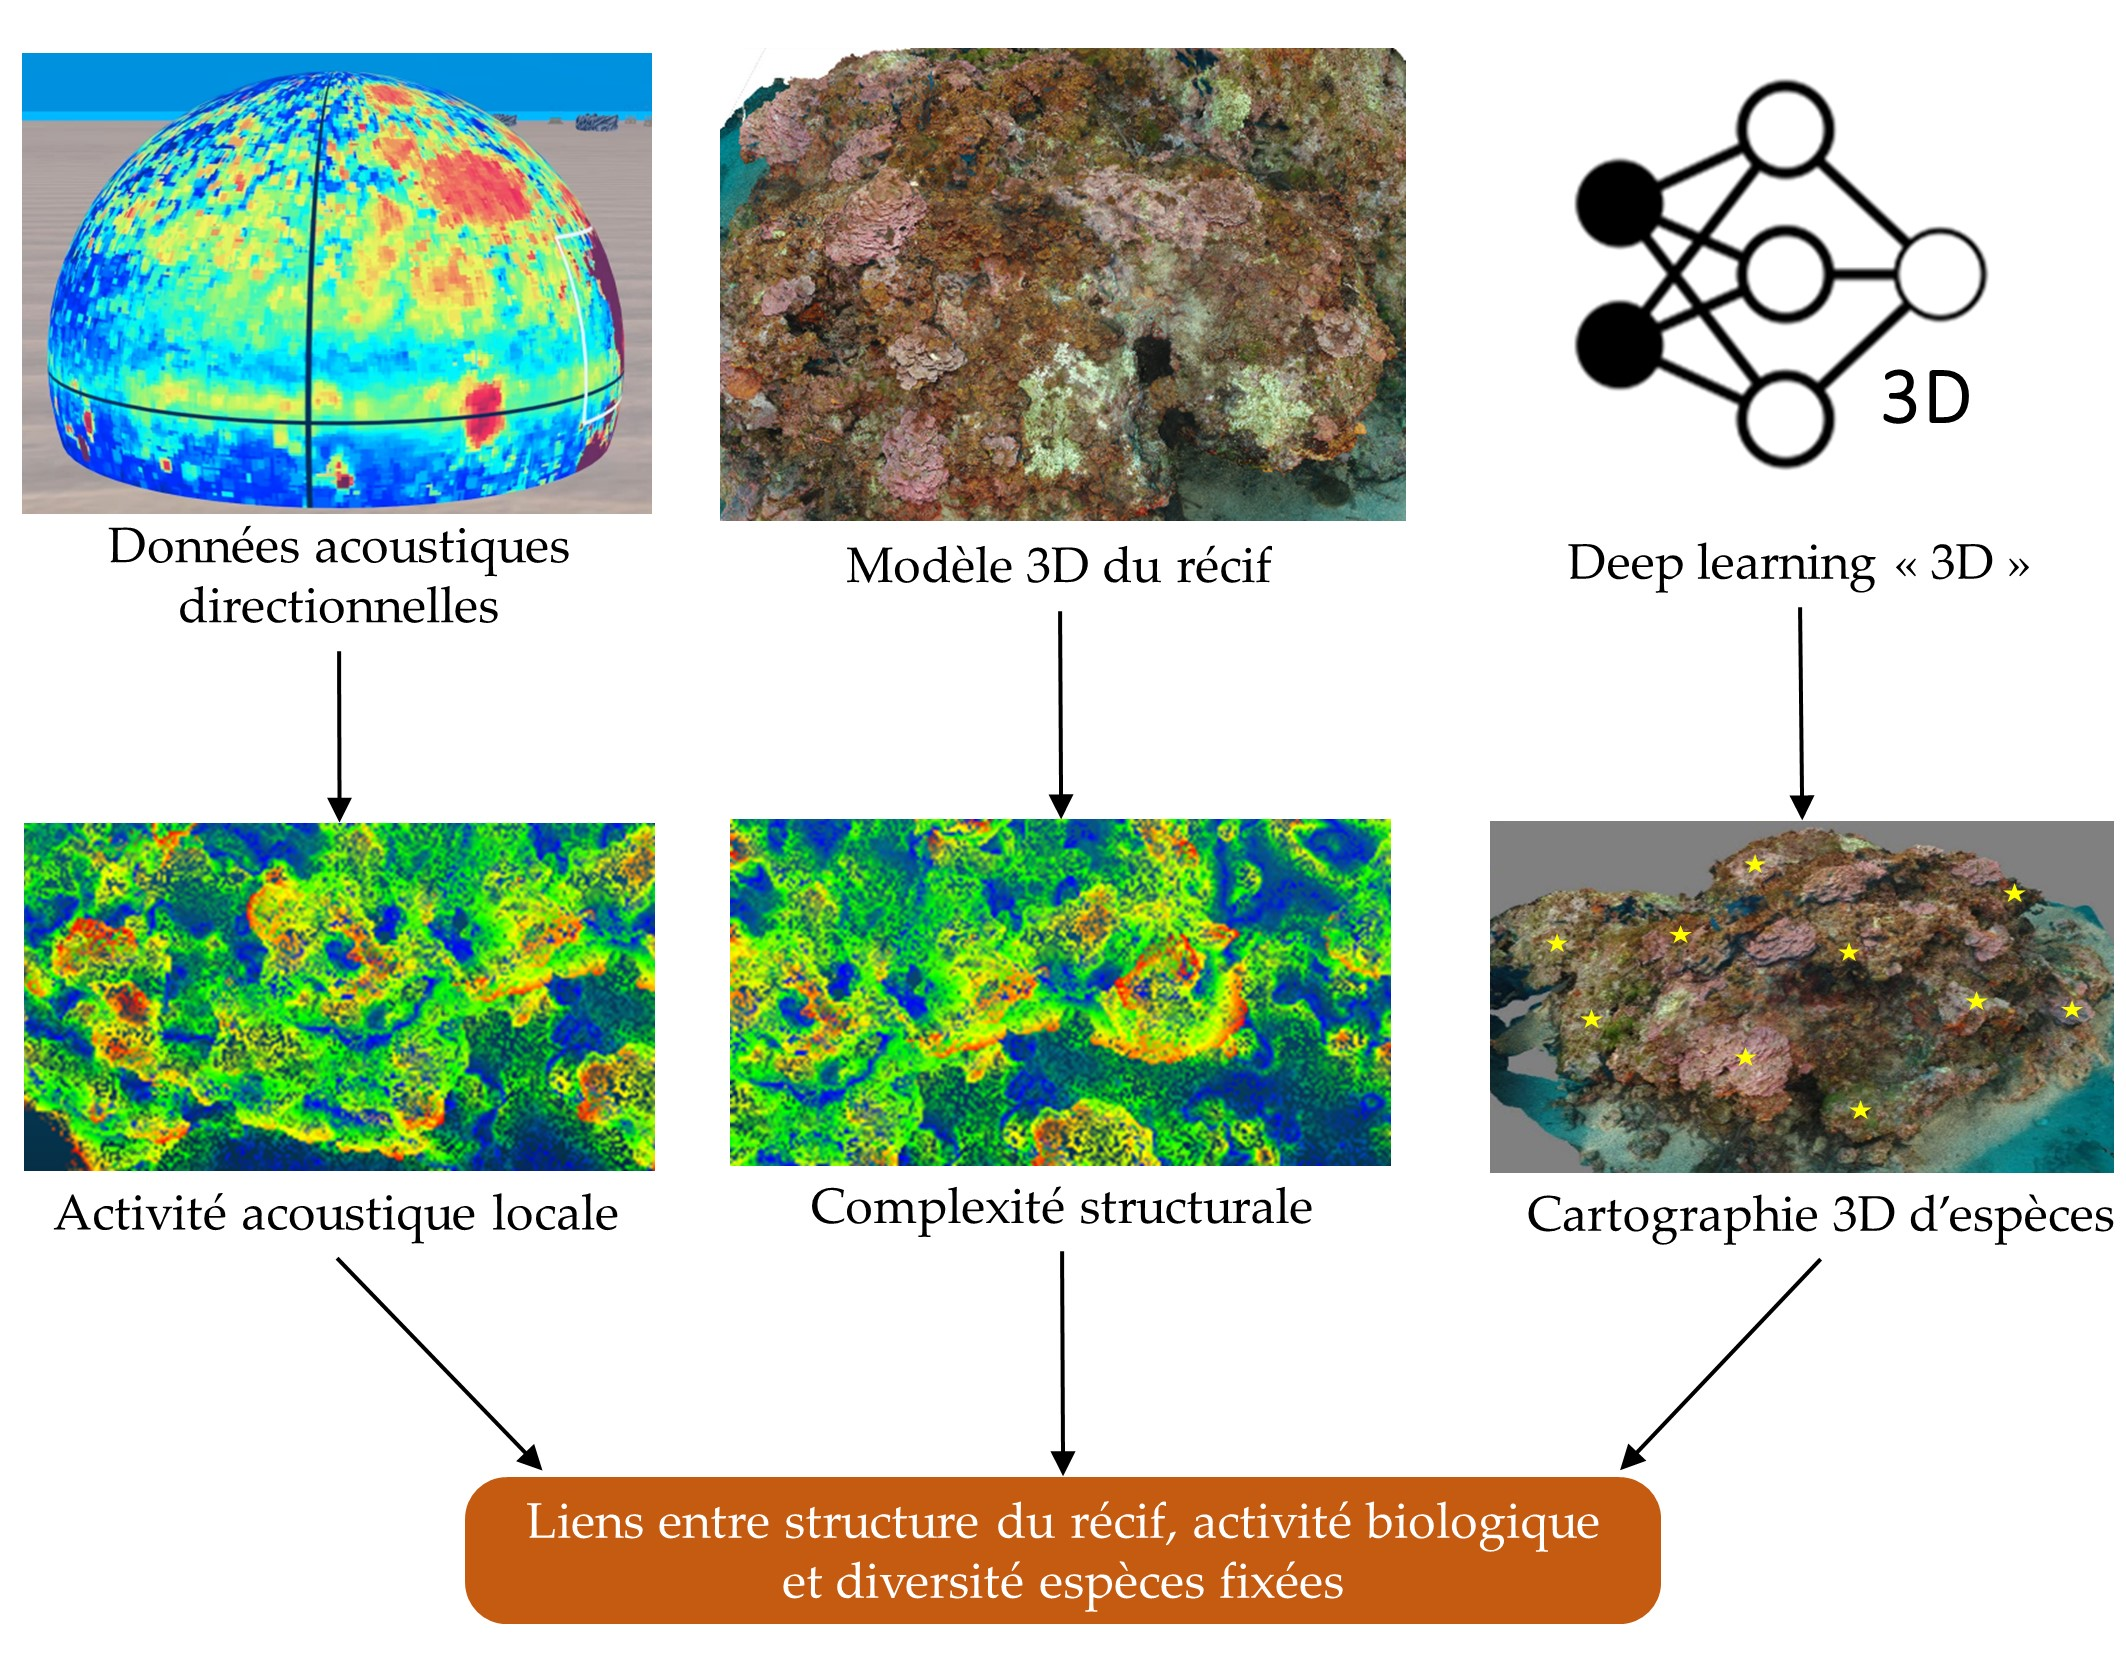
\includegraphics[width=\linewidth,keepaspectratio]{./7_discussion/couplage_PG_deep_acoustique}
		\caption{Étude à fine échelle des liens entre la structure des récifs, la composition des assemblages fixés et les espèces mobiles.}
	\label{figure_discussion6}
\end{center}
\end{figure}

\subsection{Suivis photogrammétriques de zones de grande étendue}

Si les modèles 3D utilisés dans ce travail de recherche couvraient des surfaces de l’ordre de quelques dizaines à quelques centaines de mètres carrés, certaines études pourraient nécessiter de cartographier une zone plus large encore. Toutefois, sans positionnement GPS et dans des conditions de visibilité bien souvent limitées, il n’est pas évident pour le plongeur de conserver une trajectoire optimale et un recouvrement latéral suffisant pour assurer une bonne acquisition photogrammétrique et une reconstruction 3D de qualité. Il est donc impératif de relever régulièrement des repères visuels et de s’aider d’un compas pour limiter ces écarts à la trajectoire, mais dans les cas les plus difficiles, il n’est pas rare de passer deux fois au même endroit, ou à l’inverse d’avoir une couverture insuffisante à certains endroits. Cela est d’autant plus vrai que la surface à couvrir est grande, car toute dérive dans la trajectoire devient vite importante. C’est pourquoi dans le cadre du laboratoire commun InToSea porté par Andromède Océanologie et l’UMR MARBEC (\href{https://labcomintosea.edu.umontpellier.fr}{https://labcomintosea.edu.umontpellier.fr}), nous avons engagé le développement d’un outil d’acquisition plongeur, permettant de réaliser les images et de visualiser leur alignement et le nuage de points 3D en temps réel (\autoref{figure_discussion7}). 

%%%%%%%%%%%%%%%%%%%%%%%%%%%%%%%%%%%%%%%%%%%%%%%%%%%
%%% Figure discussion 7: outil plongeur %%%
%%%%%%%%%%%%%%%%%%%%%%%%%%%%%%%%%%%%%%%%%%%%%%%%%%%
\begin{figure}[H]
	\begin{center}
	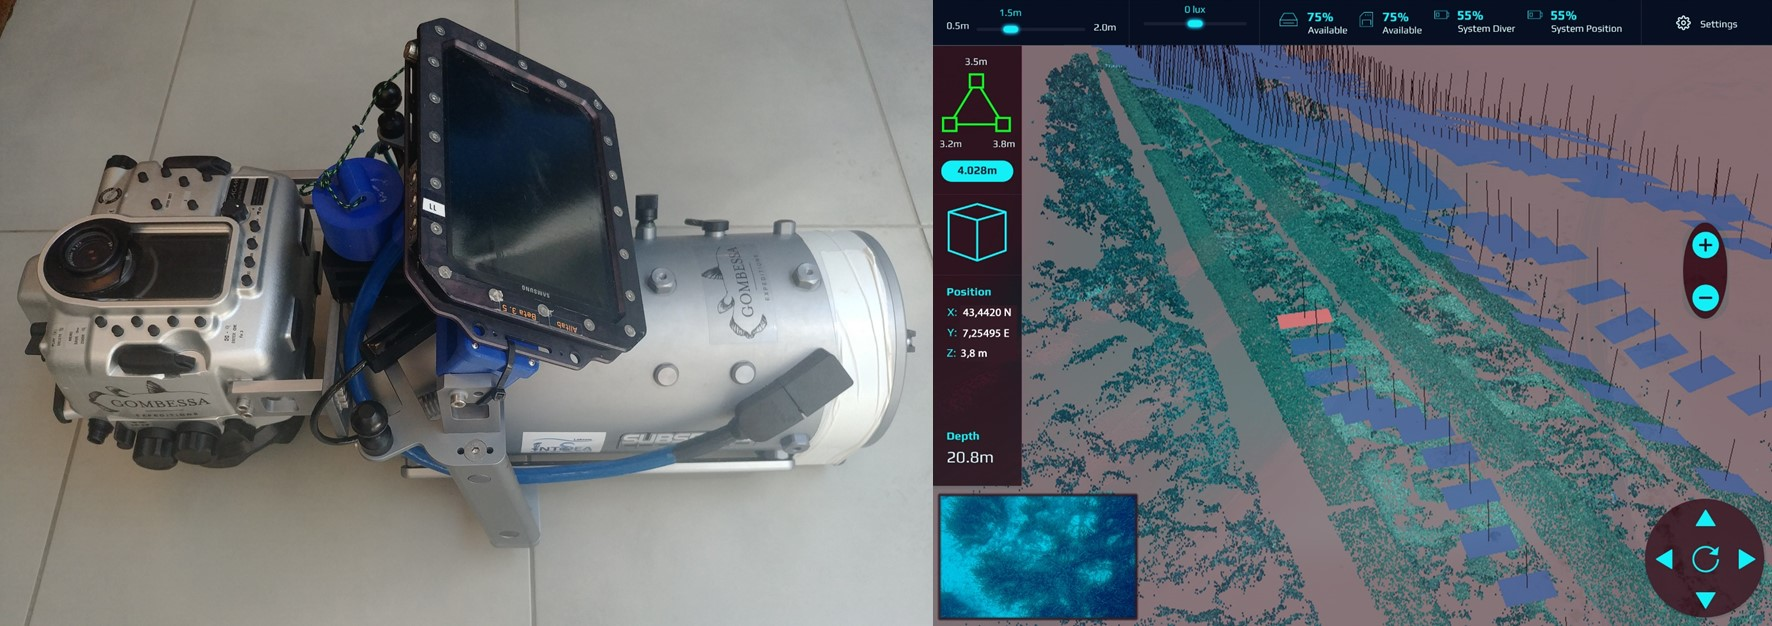
\includegraphics[width=\linewidth,keepaspectratio]{./7_discussion/outil_plongeur}
		\caption[Prototype d’acquisition plongeur permettant de réaliser l’alignement des images en temps réel]{Prototype d’acquisition plongeur permettant de réaliser l’alignement des images en temps réel. À gauche : le prototype ; à droite : exemple d’affichage tablette au cours d’une acquisition.}
	\label{figure_discussion7}
\end{center}
\end{figure}

Le prototype est constitué d’un Nikon D4 pour les prises de vue, d’une tablette Android pour la visualisation, et d’un ordinateur de bord doté d’une puissante carte graphique pour l’alignement en temps réel des images (ordinateur et batteries logés dans un caisson étanche Subspace). Le système utilise l’alignement séquentiel d’images rendu possible avec PhotoScan pour déterminer la position et l’orientation des images relativement à notre mire et ses quatre cardinales (voir Méthodes section 2.4.2), automatiquement détectées par PhotoScan. Il est ainsi possible de surveiller sa trajectoire, vérifier que l’alignement se déroule correctement et de facilement se localiser dans l’espace, y compris par visibilité réduite. Le prototype, développé par Benoît Ropars (labcom IntoSea), est en cours de finalisation suite à des modifications matérielles et devrait être opérationnel à l’automne 2020.

\subsection{Application des méthodes à d’autres habitats marins}

Si l’objectif de ce travail de thèse était de répondre aux besoins des réseaux de surveillance TEMPO (herbiers de posidonie) et RECOR (récifs coralligènes) en Méditerranée française, qui ont par ailleurs facilité l’accès aux bases de données existantes et l’acquisition de nouvelles données, ces méthodes ne sont pas intégralement spécifiques à ces deux habitats et sont en partie transférables à d’autres écosystèmes. En effet, comme mentionné en discussion du chapitre 3, la méthode de cartographie des herbiers basée sur le nuage de points épars pourrait être adaptée à d’autres habitats en ajustant les paramètres. Il serait ainsi envisageable de cartographier d’autres types de végétation sous-marine comme les herbiers de zostère (Zostera noltei, liste rouge IUCN), de cymodocée (Cymodocea nodosa, liste rouge IUCN) ou encore les algues qui colonisent les récifs coralliens. Par ailleurs, la photogrammétrie est déjà assez largement utilisée en milieu corallien pour réaliser des mesures morphologiques à l’échelle de la colonie \citep{courtney_estimating_2007, agudo-adriani_colony_2016, zawada_quantifying_2019} comme du récif \citep{leon_measuring_2015, burns_assessing_2016, bryson_characterization_2017, pizarro_simple_2017, anelli_towards_2019}. Grâce aux compétences acquises en photogrammétrie sous-marine au cours de ce travail de thèse, depuis l’acquisition jusqu’au traitement des modèles 3D, Andromède Océanologie a remporté un projet de suivi de croissance de boutures de corail sur des récifs artificiels aux Philippines, sur l’île de Pangatalan (\autoref{figure_discussion8}). Ce projet comporte plusieurs suivis à différentes échelles, de la croissance à l’échelle des boutures jusqu’à la dynamique morphologique du récif restauré. Enfin, un inventaire et un suivi de colonies de corail rouge doivent démarrer en juillet 2020 dans le Parc naturel marin du cap Corse et de l’Agriate.

%%%%%%%%%%%%%%%%%%%%%%%%%%%%%%%%%%%%%%%%%%%%%%%%%%%
%%% Figure discussion 8: autres habitats %%%
%%%%%%%%%%%%%%%%%%%%%%%%%%%%%%%%%%%%%%%%%%%%%%%%%%%
\begin{figure}[H]
	\begin{center}
	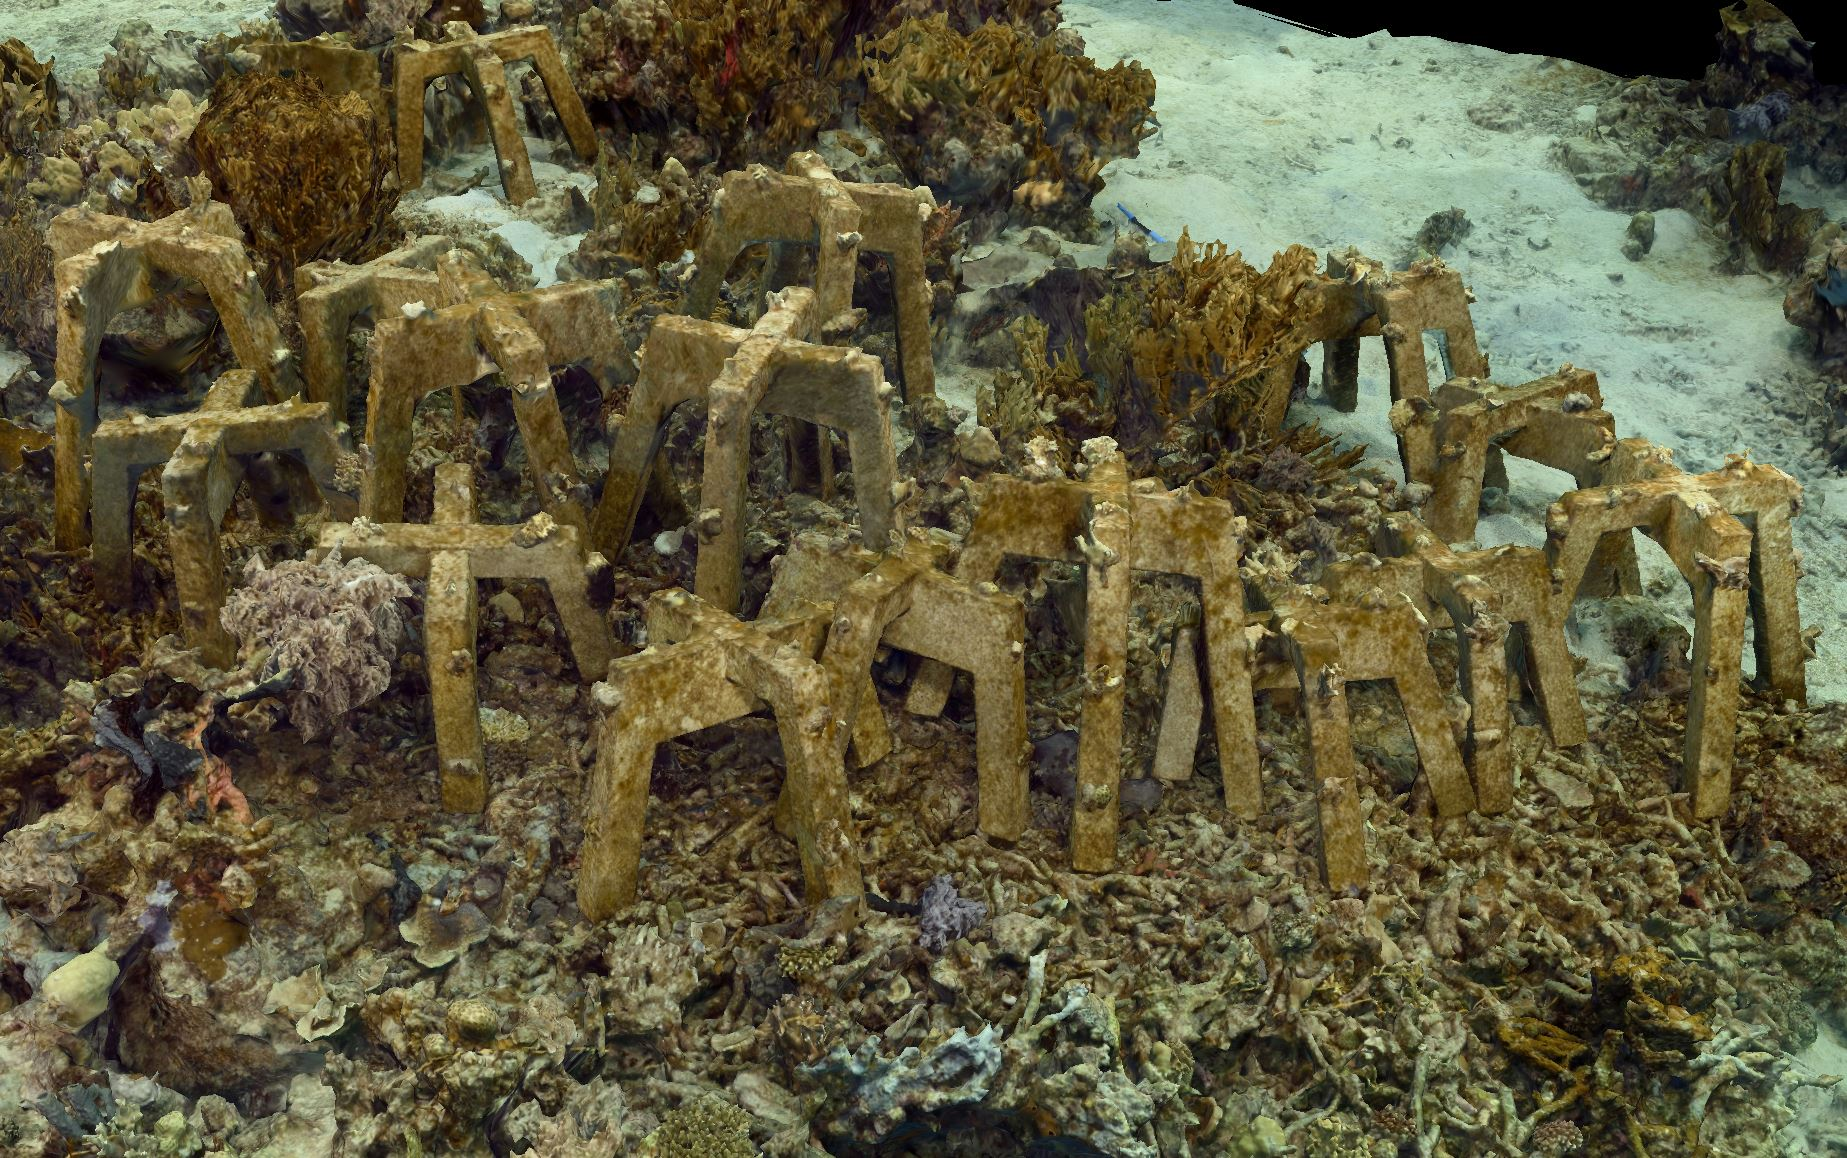
\includegraphics[width=\linewidth,keepaspectratio]{./7_discussion/SRP}
		\caption{Modèle 3D de supports de boutures de corail à Pangatalan (Philippines).}
	\label{figure_discussion8}
\end{center}
\end{figure}

\newpage

\section{Conclusion}\label{discussion.4}

Le travail réalisé au cours de cette thèse a permis de répondre à certains besoins de la surveillance et de la conservation des habitats marins en fournissant des \textbf{outils d’évaluation de la biodiversité} et de l\textbf{’état écologique} de deux habitats sensibles en Méditerranée : les \textbf{herbiers de posidonie} et les\textbf{ récifs coralligènes}. En particulier, nous avons développé des méthodes opérationnelles de suivis de la biodiversité de ces deux habitats, basées sur \textbf{deux techniques d’analyse d’images} : les \textbf{réseaux de neurones convolutifs} et la \textbf{photogrammétrie}. Ces méthodes permettent de suivre efficacement et précisément \textbf{l’état de santé} des habitats marins et les \textbf{services écosystémiques} qu’ils fournissent, malgré les contraintes du milieu marin.

Cette thèse a prouvé la capacité des réseaux de neurones à \textbf{reconnaître les principales espèces} du coralligène sur des quadrats photographiques, ouvrant ainsi la voie à l’automatisation de cette tâche chronophage et permettant d’\textbf{intensifier l’effort d’échantillonnage} sur ces récifs dont la composition écologique est très variable dans l’espace. Par ailleurs, nous avons démontré la \textbf{faisabilité} d’utiliser la photogrammétrie pour suivre des habitats benthiques, en particulier pour \textbf{cartographier} les herbiers de posidonie et \textbf{étudier la structure} des récifs coralligènes.

D’autre part, cette thèse a également ouvert de nouvelles \textbf{perspectives de recherche}, potentielles futures études en collaboration avec Andromède Océanologie. Par exemple, la caractérisation à plus fine échelle des \textbf{liens entre la structure} et les \textbf{assemblages coralligènes} en cartographiant la position des espèces sur le modèle 3D. En outre, ce travail n’a pas pris en compte le \textbf{compartiment mobile} dans les évaluations écologiques (poissons, invertébrés benthiques…), mais l’association de \textbf{plusieurs méthodes innovantes} incluant celles présentées dans ce manuscrit pourrait permettre d’étudier ces relations. Enfin, un transfert de méthodes sur d’autres habitats comme les \textbf{récifs coralliens} ouvrirait des perspectives de surveillance en dehors de la Méditerranée.

Dans le contexte de changement global actuel où il est indispensable d’étudier et de suivre les \textbf{dynamiques spatio-temporelles} de la \textbf{biodiversité marine} afin de mieux les comprendre et mettre en place des \textbf{mesures de conservation}, les résultats obtenus et les perspectives soulevées durant ce travail doctoral contribuent à répondre aux \textbf{Objectifs de Développement Durable pour 2030} (Biodiversity and the 2030 Agenda for Sustainable Development). 